\documentclass[a4paper,12pt]{extarticle}
\usepackage[utf8x]{inputenc}
\usepackage[T1,T2A]{fontenc}
\usepackage[russian]{babel}
\usepackage[hidelinks]{hyperref}
\usepackage{indentfirst}
\usepackage{listings}
\usepackage{color}
\usepackage{here}
\usepackage{array}
\usepackage{multirow}
\usepackage{graphicx}
\usepackage{subcaption} 
\usepackage{mathtools}
\usepackage{listings}

\usepackage{caption}
\renewcommand{\lstlistingname}{Программа} % заголовок листингов кода

\bibliographystyle{ugost2008ls}

\usepackage{listings}
\lstset{ %
extendedchars=\true,
keepspaces=true,
language=C,						% choose the language of the code
basicstyle=\footnotesize,		% the size of the fonts that are used for the code
numbers=left,					% where to put the line-numbers
numberstyle=\footnotesize,		% the size of the fonts that are used for the line-numbers
stepnumber=1,					% the step between two line-numbers. If it is 1 each line will be numbered
numbersep=5pt,					% how far the line-numbers are from the code
backgroundcolor=\color{white},	% choose the background color. You must add \usepackage{color}
showspaces=false				% show spaces adding particular underscores
showstringspaces=false,			% underline spaces within strings
showtabs=false,					% show tabs within strings adding particular underscores
frame=single,           		% adds a frame around the code
tabsize=2,						% sets default tabsize to 2 spaces
captionpos=t,					% sets the caption-position to top
breaklines=true,				% sets automatic line breaking
breakatwhitespace=false,		% sets if automatic breaks should only happen at whitespace
escapeinside={\%*}{*)},			% if you want to add a comment within your code
postbreak=\raisebox{0ex}[0ex][0ex]{\ensuremath{\color{red}\hookrightarrow\space}},
texcl=true,
inputpath=listings,                     % директория с листингами
}

\usepackage[left=2cm,right=2cm,
top=2cm,bottom=2cm,bindingoffset=0cm]{geometry}

%% Нумерация картинок по секциям
\usepackage{chngcntr}
\counterwithin{figure}{section}
\counterwithin{table}{section}

%%Точки нумерации заголовков
\usepackage{titlesec}
\titlelabel{\thetitle.\quad}
\usepackage[dotinlabels]{titletoc}

%% Оформления подписи рисунка
\addto\captionsrussian{\renewcommand{\figurename}{Рисунок}}
\captionsetup[figure]{labelsep = period}

%% Подпись таблицы
%\DeclareCaptionFormat{hfillstart}{\hfill#1#2#3\par}
%\captionsetup[table]{format=hfillstart,labelsep=newline,justification=centering,skip=-10pt,textfont=bf}

%% Путь к каталогу с рисунками
\graphicspath{{fig/}}

%% Внесение titlepage в учёт счётчика страниц
\makeatletter
\renewenvironment{titlepage} {
 \thispagestyle{empty}
}
\makeatother

\DeclarePairedDelimiter\abs{\lvert}{\rvert}%
\DeclarePairedDelimiter\norm{\lVert}{\rVert}%

\usepackage{amsmath}

\begin{document}	% начало документа

% Титульная страница
\begin{titlepage}	% начало титульной страницы

	\begin{center}		% выравнивание по центру

		\large Санкт-Петербургский политехнический университет Петра Великого\\
		\large Институт прикладной математики и механики \\
		\large Кафедра <<Прикладная математика>>\\[6cm]
		% название института, затем отступ 6см
		
		%\huge Математическая статистика\\[0.5cm] % название работы, затем отступ 0,5см
		\huge Методы оптимизации\\[0.5cm] % название работы, затем отступ 0,5см
		%\large \textbf{Отчет по лабораторной работе №4}\\[5.1cm]
		\large \textbf{Отчет по лабораторной работе \\``Решение задач одномерной минимизации ``}\\[5.1cm]
		%\\[5cm]

	\end{center}


	\begin{flushright} % выравнивание по правому краю
		\begin{minipage}{0.25\textwidth} % врезка в половину ширины текста
			\begin{flushleft} % выровнять её содержимое по левому краю

				\large\textbf{Работу выполнил:}\\
				\large Колесник В.Н.\\
				\large {Группа:} 3630102/70201\\
				
				\large \textbf{Преподаватель:}\\
				\large к.ф.-м.н., доцент\\
				%\large Баженов Александр Николаевич
				\large Родионова Елена Александровна

			\end{flushleft}
		\end{minipage}
	\end{flushright}
	
	\vfill % заполнить всё доступное ниже пространство

	\begin{center}
	\large Санкт-Петербург\\
	\large \the\year % вывести дату
	\end{center} % закончить выравнивание по центру

\end{titlepage} % конец титульной страницы

\vfill % заполнить всё доступное ниже пространство


% Содержание
\renewcommand\contentsname{\centerline{Содержание}}
\tableofcontents
\newpage

\listoffigures

\newpage

%\listoftables

%\newpage

\section{Постановка задачи}
В двумерном пространстве имеется Г-образный канал заданной ширины. Задана конфигурация двумерного жёсткого тела (плота): прямоугольник с вырезом-сегментом круга на одной из сторон. \\
Необходимо подобрать такие параметры размеров плота, чтобы он мог пройти через канал и имел наибольшую площадь.


\section{Формализация задачи}
\subsection{Канал}
Заданная ширина канала - 1. \\

Введем декартову систему координат и разместим начало отсчета в ``дальнем`` углу канала. Орты будут проходить вдоль стен. Тогда свободную область канала можно представить следующим множеством:\\
\begin{equation}
\Omega=\{(x,y) | 0\leq x \leq 1 ; 0\leq y \leq 1\} \cup \{(x,y) | 1 \leq x ; 0\leq y \leq 1\} \cup \{(x,y) | 0\leq x \leq 1 ; 1 \leq y \}
\end{equation}
Для удобства будем называть угол $(1,1)$ ближним, а угол $(0,0)$ - дальним.

\begin{figure}[!htb]
    \centering
    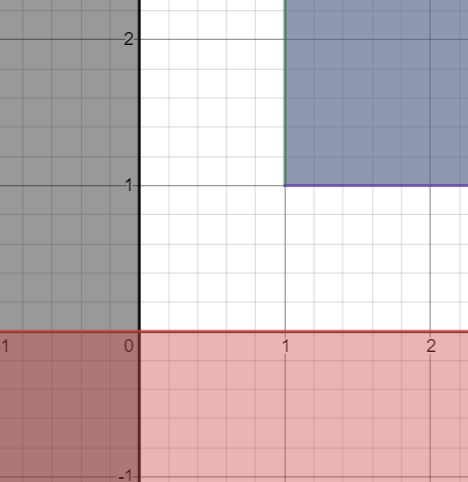
\includegraphics[width=0.5\textwidth]{fig/corridor.png}
    \caption{Канал}
\end{figure}


\subsection{Плот}
Плот представляет собой прямоугольник с вырезом в виде сегмента круга на одной из сторон. Иначе говоря, плот является результатом разности множества Прямоугольник и множества Круг. \\

Одна пара сторон, которую не касается вырез, имеет фиксированную длину, равную ширине канала - 1. \\

Длину другой пары сторон нужно изменять для решения задачи. Обозначим ее как $b$. \\ 

Окружность для выреза обязана проходить через 2 угла прямоугольника и делать вырез со стороны не фиксированной длины. Другими словами, стороны фиксированной длины не могут быть обрезаны по длине данным кругом. Позицию центра круга будем определять по длине отрезка от стороны, параллельной обрезанной стороне, до центра круга. Эту длину обозначим за $c$. \\

Назовем характерные точки $A$, $B$, $C$ (они отмечены на рисунке).\\

Тогда радиус круга будет равен:
\begin{equation}
R=\sqrt{(c-1)^2+\frac{b^2}{4}}
\end{equation}

Площадь плота может быть посчитана так:
\begin{equation}
S=b-(\frac{2\pi ((c-1)^2+\frac{b^2}{4})}{360} \arctan{\frac{b}{2(c-1)}} - \frac{b}{2}(c-1))
\end{equation}

\begin{figure}[!htb]
    \centering
    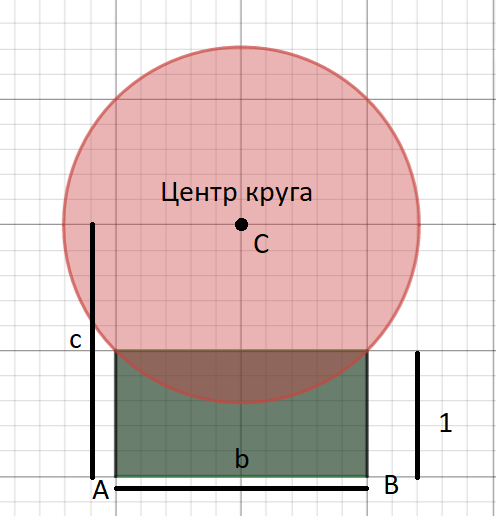
\includegraphics[width=0.4\textwidth]{fig/sofa.png}
    \caption{Плот}
\end{figure}


\subsection{Движение плота}
На рисунке не будут отмечены боковые стороны плота длины 1. Далее будет пояснено, почему они не влияют на проходимость плота. Вырез обозначен окружностью с центром $C$. Необрезанная сторона $AB$ представлена красным отрезком. Точка $A$ - синяя, точка $B$ - красная.\\

Будем считать, что движение плота происходит следующим образом:
\begin{itemize}
\item Плот движется по коридору вырезом в сторону ближнего угла, необрезанной стороной $AB$ к стене $x=0$. Так как длина боковых сторон равна ширине канала, то плот спокойно сможет пройти до дальнего угла. В конце такого прямолинейного движения координаты точек $A$ и $B$ будут $(0,0)$ и $(b,0)$ соответственно.
\begin{figure}[!htb]
    \centering
    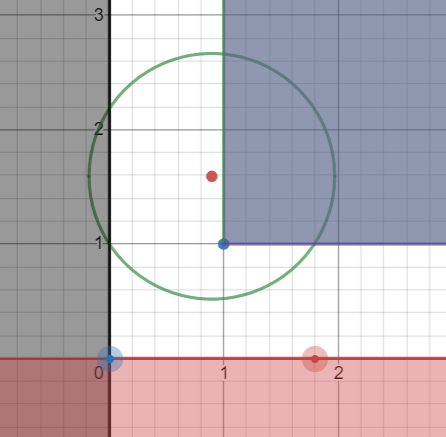
\includegraphics[width=0.4\textwidth]{fig/sofa1.png}
    \caption{Начало движения}
\end{figure}

\newpage

\item Далее плот совершает поворот, не отрывая сторону $AB$ от стен дальнего угла. То есть должны выполняться следующие условия: $A_x=0$, $B_y=0$. Вырез же должен помочь обойти ближний угол. \\
Так как длина боковых сторон плота равна ширине канала, то при повороте эти стороны гарантировано смогут пройти. Плот касается стен только в 2 или 3 местах: точки $A$, $B$ и, быть может, вырез. Поэтому боковые стороны можно игнорировать.
\begin{figure}[!htb]
    \centering
    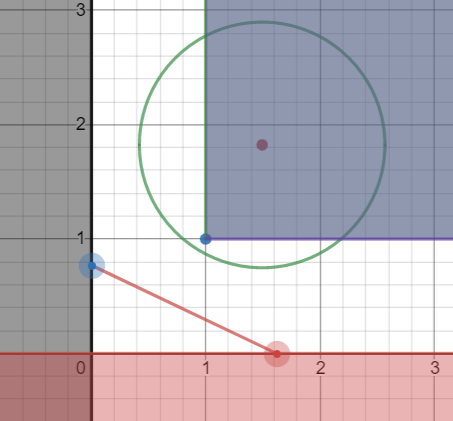
\includegraphics[width=0.4\textwidth]{fig/sofa2.png}
    \caption{Поворот}
\end{figure}

\newpage

\item После такого поворота плот должен оказаться в положении, аналогичном началу движения. По причинам, указанным в 1 пункте, он сможет свободно пройти по каналу.
\begin{figure}[!htb]
    \centering
    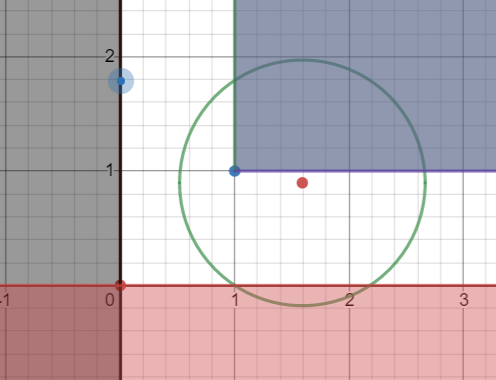
\includegraphics[width=0.4\textwidth]{fig/sofa3.png}
    \caption{Конец движения}
\end{figure}

\end{itemize}

Таким образом, основной проблемой является только поворот плота. Формализуем это движение. Зададим параметр времени $t \in [0;1]$, где время $t=0$ соответствует началу поворота, а время $t=1$ - концу поворота. \\

Тогда движение точек можно описать так:
\begin{equation}
A_x = 0; A_y=tb
\end{equation}
\begin{equation}
B_x = b\sqrt{1-t^2}; B_y=0
\end{equation}
\begin{equation}
C_x = \frac{b\sqrt{1-t^2}}{2}+tc; C_y=\frac{bt}{2}+c\sqrt{1-t^2}
\end{equation}


\subsection{Ограничения на параметры плота}
Очевидно, что самая простая версия плота - квадрат со сторонами 1 - сможет пройти по каналу без поворота (формально: $b=1$, центр круга бесконечно удален). Поэтому сторону b можно ограничить снизу значением 1. \\

Чтобы сторона $AB$ не пересекала стены ближнего угла при повороте, нужно ограничить ее длину сверху значением $2\sqrt{2}$ (это число можно получить из уравнения прямой, проходящей через точки $A$ и $B$, когда плот совершил половину поворота). \\

На круг для выреза накладывается следующее ограничение: центр круга не может находиться в прямоугольник. Поэтому для $c$ получаем оценку снизу - 1. \\

Кроме того, вырез не должен заходить на стены ближнего угла. Для этого ограничим расстояние от центра круга до ближнего угла $(1,1)$ сверху радиусом этого круга. То есть при повороте ближний угол должен находиться в круге. \\

Таким образом, получаем следующие ограничения:
\begin{equation}
1 \leq b \leq 2\sqrt{2}
\end{equation}
\begin{equation}
1 \leq c
\end{equation}
\begin{equation}
( \frac{b\sqrt{1-t^2}}{2}+tc - 1)^2 + (\frac{bt}{2}+c\sqrt{1-t^2}-1)^2 \leq (c-1)^2+\frac{b^2}{4}
\end{equation}

\subsection{Задача}
Формально задачу можно представить так:
\begin{equation}
b-(\frac{2\pi ((c-1)^2+\frac{b^2}{4})}{360} \arctan{\frac{b}{2(c-1)}} - \frac{b}{2}(c-1)) \rightarrow max
\end{equation}
\begin{equation}
1 \leq b \leq 2\sqrt{2}
\end{equation}
\begin{equation}
1 \leq c
\end{equation}
\begin{equation} \label{center}
( \frac{b\sqrt{1-t^2}}{2}+tc - 1)^2 + (\frac{bt}{2}+c\sqrt{1-t^2}-1)^2 \leq (c-1)^2+\frac{b^2}{4}, \forall t \in [0;1]
\end{equation}



\section{Упрощение задачи}
\subsection{Избавление от параметра времени}
Параметр времени $t$ в задаче присутствует только в одном ограничении - (\ref{center}). Имеет смысл заменить это условие равносильным без использования параметра. \\

Попробуем найти такое $t$, при котором левая часть при фиксированных $c$ и $b$ будет наибольшей. Тогда можно будет это наибольшее сравнивать с правой частью, которая не зависит от $t$. \\
\textbf{Утверждение}\\
Левая часть неравенства (\ref{center}) достигает наибольшего значения при $t=\frac{1}{\sqrt{2}}$ для фиксированных $c$ и $b$, для которых не выполнено условие $2 b (\sqrt{2} - 4 c) + 4 \sqrt{2} c \geq 0$\\
\textbf{Доказательство}\\
Рассмотрим левую часть неравенства, как функцию 1 переменной:
\begin{equation}
f(t)=( \frac{b\sqrt{1-t^2}}{2}+tc - 1)^2 + (\frac{bt}{2}+c\sqrt{1-t^2}-1)^2, \forall t \in [0;1]
\end{equation}
\begin{equation}
f'(t)=2( \frac{b\sqrt{1-t^2}}{2}+tc - 1)(-\frac{bt}{2\sqrt{1-t^2}}+c)+2(\frac{bt}{2}+c\sqrt{1-t^2}-1)(\frac{b}{2}-\frac{ct}{\sqrt{1-t^2}})
\end{equation}
\begin{equation}
f'(\frac{1}{\sqrt{2}})=2( \frac{b}{2\sqrt{2}}+\frac{c}{\sqrt{2}} - 1)(-\frac{b}{2}+c)+2(\frac{b}{2\sqrt{2}}+\frac{c}{\sqrt{2}}-1)(\frac{b}{2}-c)=0
\end{equation}
\begin{equation}
f''(\frac{1}{\sqrt{2}})=2 b (\sqrt{2} - 4 c) + 4 \sqrt{2} c < 0
\end{equation}
\begin{equation}
c>\frac{b}{\sqrt{2}(2b-\sqrt{2})}; b\in[1;2\sqrt{2}]
\end{equation}
По условиям задачи $b$ ограничено сверху и снизу. Для всех значений $b$ правая часть неравенства является конечным положительным числом. Так как $c$ сверху не ограничено, то найдется такой значение, для которого неравенство будет выполняться. Оно также будет выполняться для всех больших значений $c$. Значит, множество значений $b$ и $c$, при котором вторая производная отрицательна, непусто. Его можно описать так:
\begin{equation}
S=\{(b,c) | b \in [1;2\sqrt{2}]; max(1,\frac{b}{\sqrt{2}(2b-\sqrt{2})}) \leq c \}
\end{equation}
Так как первая производная равна нулю в точке $t=\frac{1}{\sqrt{2}}$, а вторая производная отрицательна, выполнено достаточное условие максимума. \\
Значит, в $t=\frac{1}{\sqrt{2}}$ левая часть неравенства (\ref{center}) достигает наибольшего значения. \\

\textbf{Замечание}\\
Значение $t=\frac{1}{\sqrt{2}}$ соответствует половине поворота плота. Иначе говоря, ближний угол канала находится ближе всего к обрезаннной стороне тогда, когда $A_y=B_x$.

\textbf{Замечание}\\
Рассмотрим область, которую не охватывает утверждение. По оси $x$ отложены значения $b$, по оси $y$ - $c$.
\begin{equation}
D=\{(b,c) | b \in [1;2\sqrt{2}]; 1 \leq c \leq \frac{b}{\sqrt{2}(2b-\sqrt{2})}\}
\end{equation}

\begin{figure}[!htb]
    \centering
    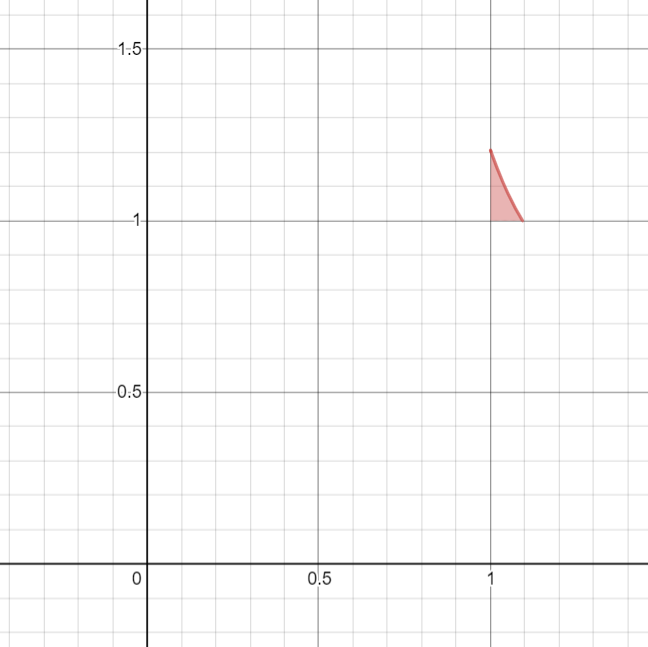
\includegraphics[width=0.4\textwidth]{fig/exception.png}
    \caption{Область $D$}
\end{figure}

Из графика видно, что для плотов с параметрами $b$ и $c$ из области $D$ эти значения близки к 1. Для таких плотов наибольшее расстояние от центра круга выреза до ближнего угла достигается не на половине поворота, а ближе к началу и концу поворота.\\

\newpage

Рассмотрим подобные плоты поподробнее. \\

\begin{figure}[!htb]
    \centering
    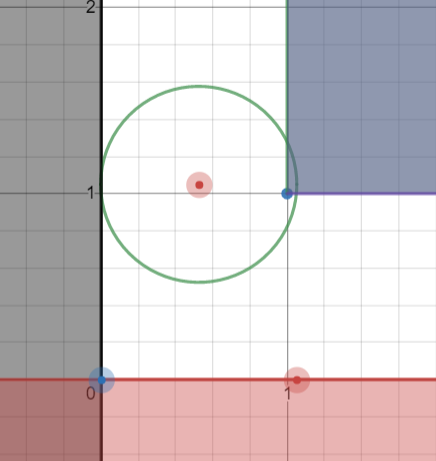
\includegraphics[width=0.4\textwidth]{fig/special.png}
    \caption{Плот с параметрами $b=1.05$, $c=1.05$}
\end{figure}

У таких плотов центр круга находится очень близко к стороне прямоугольника с вырезом. Из-за этого оказывается удалена очень большая часть прямоугольника. С таким вырезом плот точно сможет пройти по каналу. Более того, касание выреза и ближнего угла не произойдет. Поэтому при фиксированном $b$ можно попробовать поставить центр круга подальше (увеличить $c$). Тогда точка $(b,c)$ покинет область $D$ и будет выполняться утверждение. \\

Исходя из этого и упрощения, применимого в следующем пункте, можно распространить утверждение на всю область $S \cup D=\{(b,c) | 1 \leq b \leq 2\sqrt{2}, 1 \leq c \}$. \\

Поэтому можно заменить неравенство (\ref{center}) на равносильное:
\begin{equation} \label{new_center}
2( \frac{b}{2\sqrt{2}}+\frac{c}{\sqrt{2}} - 1)^2\leq (c-1)^2+\frac{b^2}{4}
\end{equation}


\subsection{Фиксирование центра круга}
Очевидно, что при фиксированной ширине плота $b$ увеличение $c$ увеличит площадь плота. Поэтому, имеет смысл для каждого $b$ выбирать максимально возможное $c$. В предыдущем пункте было показано, что ближе всего сторона с вырезом оказывается к ближнему углу канала на половине поворота плота. Значит, в остальное время движения это расстояние гарантированно будет больше. Попробуем брать такое $c$, чтобы на половине поворота плот касался ближнего угла своим вырезом. Для этого обратим неравенство (\ref{new_center}) в равенство и выразим $c$ через $b$:
\begin{equation}
2( \frac{b}{2\sqrt{2}}+\frac{c}{\sqrt{2}} - 1)^2 = (c-1)^2+\frac{b^2}{4}
\end{equation}
\begin{equation}
c=\frac{\sqrt{2}b-1}{b-2\sqrt{2}+2}
\end{equation}


\subsection{Упрощенная задача}
Таким образом, задача свелась к одномерной максимизации:
\begin{equation}
b-(\frac{2\pi ((c-1)^2+\frac{b^2}{4})}{360} \arctan{\frac{b}{2(c-1)}} - \frac{b}{2}(c-1)) \rightarrow max
\end{equation}
\begin{equation}
1 \leq b \leq 2\sqrt{2}
\end{equation}
\begin{equation}
c=\frac{\sqrt{2}b-1}{b-2\sqrt{2}+2}
\end{equation}



\section{Реализация решения задачи}
Поменяем знак целевой функции, чтобы свести задачу к одномерной минимизации:
\begin{equation}
-b+(\frac{2\pi ((c-1)^2+\frac{b^2}{4})}{360} \arctan{\frac{b}{2(c-1)}} - \frac{b}{2}(c-1)) \rightarrow min
\end{equation}
Отрезок имеет конечную длину, а функция унимодальна, что можно увидеть на графике: минимум достигается в единственной точке не на границе.\\

\begin{figure}[!htb]
    \centering
    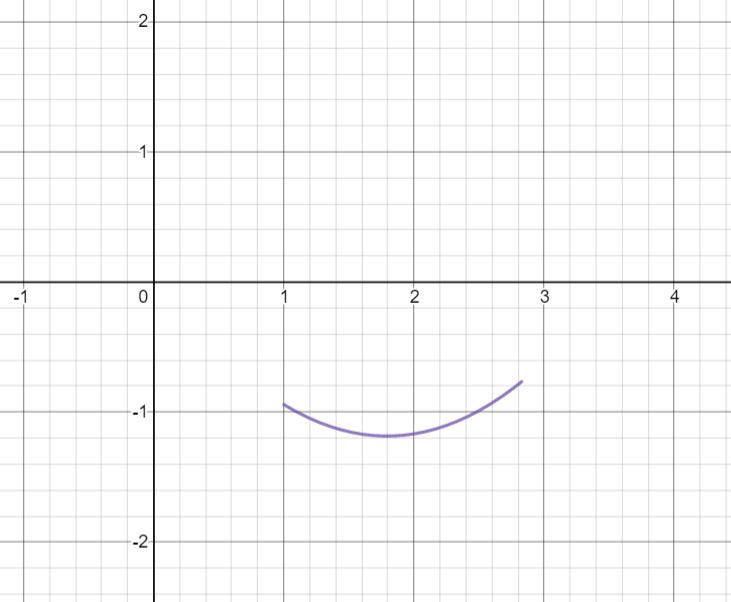
\includegraphics[width=0.4\textwidth]{fig/function.png}
    \caption{График целевой функции на отрезке $[1;2\sqrt{2}]$}
\end{figure}

Воспользуемся методом дихотомии и методом Фибоначчи с заданной точностью $\varepsilon=10^{-5}$.


\section{Результаты}
Для метода дихотомии получим интервал значений $b$ - $(1.79295, 1.79296)$. Значение функции в середине интервала равно $1.18440$. \\

Для метода Фибоначчи получим интервал значений $b$ - $(1.79296, 1.79297)$. Значение функции в середине интервала равно $1.18440$. \\

Полученная площадь плота оказалась больше, чем у простого решения с квадратным плотом. Значит, композиция увеличения ширины плота и выреза кругом помогла улучшить результат. \\

Итоговый плот представлен на картинке. По ссылкам можно посмотреть визуализацию движения плотов с разными параметрами и плота с параметром $b=1.79296$.
\begin{figure}[!htb]
    \centering
    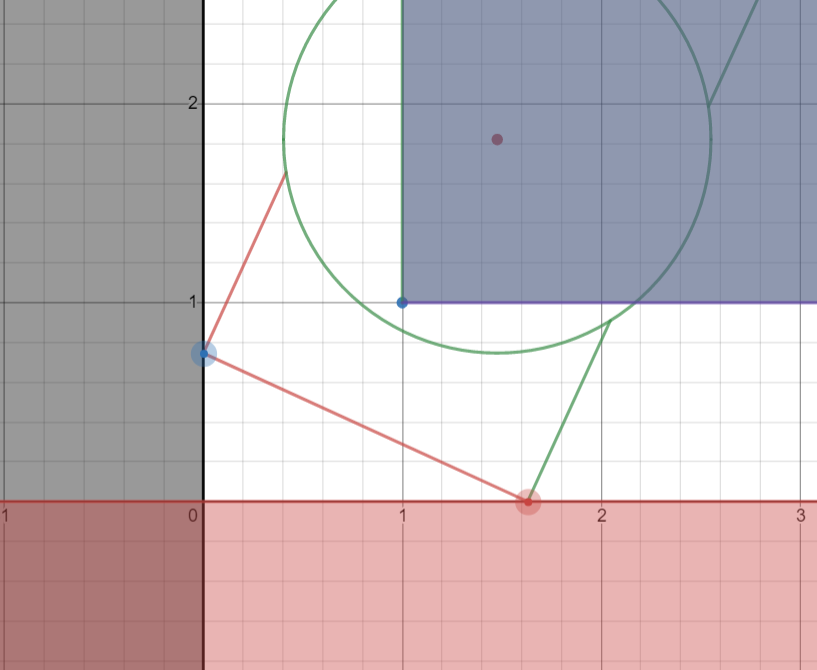
\includegraphics[width=0.4\textwidth]{fig/solution.png}
    \caption{Плот с параметром $b=1.79296$}
\end{figure}


\newpage

\section{Ссылки}
\noindent [1] Визуализация движения плотов с разной шириной \\
{\url{https://www.desmos.com/calculator/0xjd0p7hu1}} \\
\noindent [2] Визуализация движения плота с параметром $b=1.79296$ \\
{\url{https://www.desmos.com/calculator/muse239cmb}} \\
\noindent [3] Репозиторий с решением задачи \\
{\url{https://github.com/VsevolodMelnikov/Optimization/tree/master/CourseProject}}
		

\end{document}